% This LaTeX document needs to be compiled with XeLaTeX.
\documentclass[10pt]{article}
\usepackage[utf8]{inputenc}
\usepackage{ucharclasses}
\usepackage{amsmath}
\usepackage{amsfonts}
\usepackage{amssymb}
\usepackage[version=4]{mhchem}
\usepackage{stmaryrd}
\usepackage{graphicx}
\usepackage[export]{adjustbox}
\graphicspath{ {./images/} }
\usepackage{caption}
\usepackage{bbold}
\usepackage[fallback]{xeCJK}
\usepackage{polyglossia}
\usepackage{fontspec}
\IfFontExistsTF{Noto Serif CJK TC}
{\setCJKmainfont{Noto Serif CJK TC}}
{\IfFontExistsTF{STSong}
  {\setCJKmainfont{STSong}}
  {\IfFontExistsTF{Droid Sans Fallback}
    {\setCJKmainfont{Droid Sans Fallback}}
    {\setCJKmainfont{SimSun}}
}}

\setmainlanguage{english}
\setotherlanguages{dutch, polish}
\IfFontExistsTF{CMU Serif}
{\newfontfamily\lgcfont{CMU Serif}}
{\IfFontExistsTF{DejaVu Sans}
  {\newfontfamily\lgcfont{DejaVu Sans}}
  {\newfontfamily\lgcfont{Georgia}}
}
\setDefaultTransitions{\lgcfont}{}

\begin{document}
\captionsetup{singlelinecheck=false}
(0.) Being Sloppy with the constants

SOMETIMES\\
(but not always)\\
WE MAY "DROP" $\hbar$ OR $C$ OR $K_{B}$

OR WE SAY\\
$\hbar=1, C=1, K_{B}=1$\\
$\begin{array}{ccc}\uparrow & \uparrow & \uparrow \\ \text { PLANCK } & \text { SPEES } & \text { BOCTZMANN } \\ \text { CONSTANT } & \text { OF LIGHT } & \text { CONSTANT }\end{array}$\\
that is because they are not actual constants: they set a conversion rate of a unit to another

$$
\begin{aligned}
& c \simeq 3 \cdot 10^{8} \frac{m^{\leftarrow}}{s^{\leftarrow}} \overbrace{\substack{\text { UNIT OF } \\
\text { TENGTH } \\
\text { THE }}}^{\text {UNIT }} \\
& \text { Allows us to EXPRESS } \\
& \text { LENGTGS IN SECONDS } \\
& 1 \text { LEGCHS }=3.10^{8} \mathrm{~m} \\
& 47 \times \begin{array}{c}
\text { GARTH } \\
\text { RASII }
\end{array} \\
& 0.78 \times \begin{array}{c}
\text { EARTH-HOON } \\
\text { SISTANE }
\end{array} \\
& \hbar=(1.055) \cdot 10^{-34} \mathrm{Kg} \cdot \mathrm{~m}^{2} \cdot \mathrm{~s}^{-1} \\
& \text { AUOWS US TO EXPRESS } \\
& \text { HASSES IN SECONDS } \\
& 1 \text { meter }=\frac{1 / c}{3.3 \cdot 10^{-9}} \text { seconds } \\
& \frac{\hbar}{c^{2}}=1.17 \cdot 10^{-51} \frac{\mathrm{Kg}}{\mathrm{rad} / \mathrm{s}} \\
& 1 \text { "MASS" }_{\text {SECOND }}=1.17 \cdot 10^{-51} \mathrm{Kg} \\
& \xrightarrow[\text { ENERGY }]{\text { REGEST MASS }} \\
& \hbar \omega=\widetilde{m c^{2}} \\
& \hat{\mathrm{cod} / \mathrm{s}} \\
& \underset{\text { MASS }}{\text { ELECTRON }} \quad 9,11 \cdot 10^{-31} \mathrm{Kg} \\
& =7,79 \cdot 10^{20} \mathrm{rad} / \mathrm{s} \\
& (2 \pi \mathrm{~Hz}) \\
& =1.24 \cdot 10^{20} \mathrm{Mz} \text { B1E!? } \\
& \left.\begin{array}{l}
\text { COMPARE TO } \\
\text { VISIBLE LIGHT }
\end{array}\right\} \quad 4 \sim 7.9 \cdot 10^{14} \mathrm{~Hz}
\end{aligned}
$$

$K_{B}=1.38 \cdot 10^{-23} \frac{m^{2} \mathrm{Kg}}{s^{2} \mathrm{~K}}$\\
EXCERCISE. WHAT'S THE DIRECT CONVERTION RATE KELUIN-(SECOND) P?

\begin{itemize}
  \item What's the water melting temperature in (seconss)'
\end{itemize}

Careful >> not all constants are converslons, some carry acyual information

\begin{center}
\begin{tabular}{c|l}
\begin{tabular}{c}
CONVERSION \\
CONSTANTS \\
\end{tabular} & \begin{tabular}{c}
TRUE \\
CONSTANT(S) \\
\end{tabular} \\
\hline
$C$ &  \\
$\hbar$ &  \\
$K_{B}$ & $\alpha=\frac{1}{4 \pi \varepsilon_{0}} \frac{e^{2}}{\hbar c} \approx \frac{1}{137}$ \\
\begin{tabular}{c}
JUST A \\
NUMBER \\
\end{tabular} &  \\
\end{tabular}
\end{center}

\begin{center}
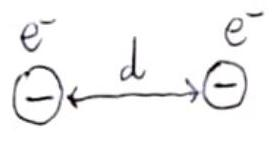
\includegraphics[max width=\textwidth]{2025_10_16_f02af6fa434c9f0bcc00g-02}
\end{center}

THERE is A specific ratio between\\
$\rightarrow$ ELECTROSTATIC ENERGY\\
$\rightarrow$ REST MASS ENERGY\\
the ratio is a function of\\
$\alpha$\\
$\left.\begin{array}{l}\text { DIFFERENT } \\ \hbar, c, K_{B}\end{array}\right\} \begin{aligned} & \text { SAME UNIVERSE } \\ & \text { DIFFERENT UNITS }\end{aligned}$\\
$\left.\begin{array}{c}\text { DIFFERENT } \\ \alpha\end{array}\right\}$ ANOTHER UNIVERSE, SIFFERENY FROM OURS

\section*{Revaew: Quantum Mech}
(1) The quantum State $\rightarrow$ (I⿴囗 POSSIBEE) TO SEFANG MEERIMINGT CALEY EVERY MGSURAALE PROPERTY OT A SYSTEM

\begin{center}
\begin{tabular}{|l|l|l|l|l|}
\hline
TAKE $\frac{\dot{x}}{\operatorname{POSITION}}$ & 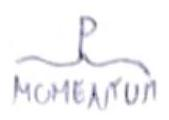
\includegraphics[max width=\textwidth]{2025_10_16_f02af6fa434c9f0bcc00g-03}
 & IF ONE IS COAPUETELY DETERMINES & $x=x_{0}$ & MSTRIBUTION $\delta\left(x-x_{0}\right)$ \\
\hline
 &  & THE OITHER ONE IS COMPEETECY UNDE TERHIVED &  & DISTRIBUTION "constant" \\
\hline
\end{tabular}
\end{center}

\begin{figure}[h]
\begin{center}
  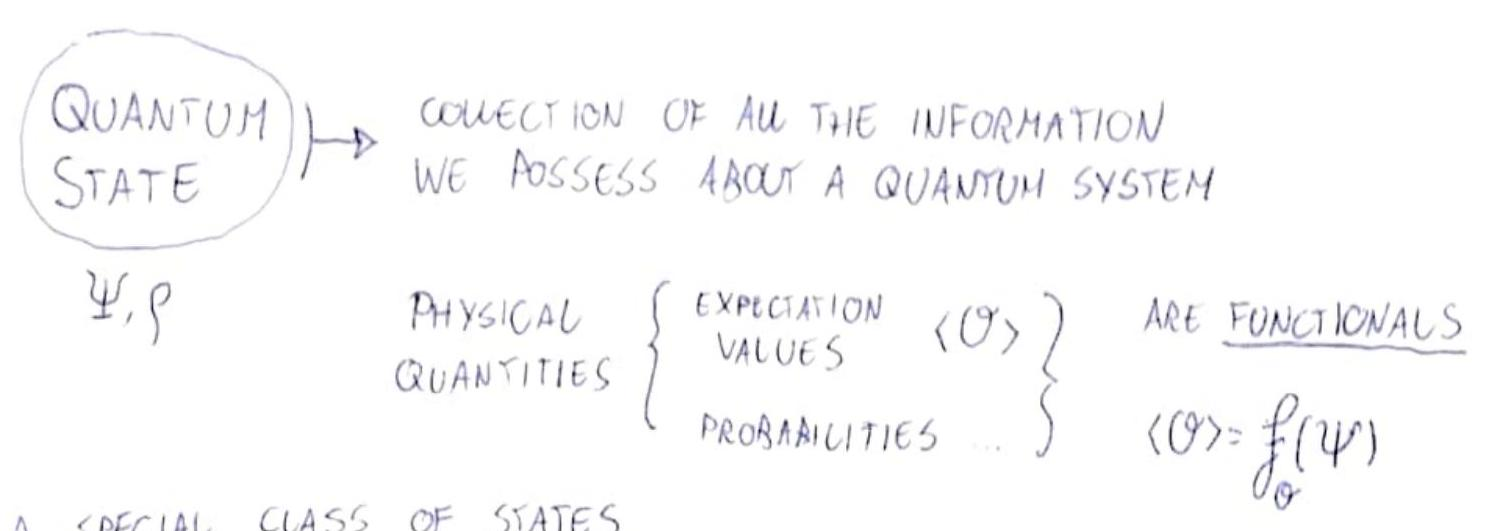
\includegraphics[width=\textwidth]{2025_10_16_f02af6fa434c9f0bcc00g-03(2)}
\captionsetup{labelformat=empty}
\caption{A SPECIAL CLASS OF STATES}
\end{center}
\end{figure}

$$
\stackrel{\text { PURE }}{\text { STATES }} \longleftrightarrow \stackrel{\text { A.K.A }}{\longleftrightarrow} \stackrel{\text { VECTOR }}{\longleftrightarrow} \frac{\text { A.K.A }}{\text { STATES }} \longleftrightarrow \text { WAVEFUNCYIONS) }
$$

are "the most deterministic" states: you can not add information WITHOUY VIOLATING SOMETHING\\
$|\psi\rangle$\\
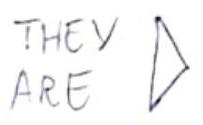
\includegraphics[max width=\textwidth, center]{2025_10_16_f02af6fa434c9f0bcc00g-03(1)}\\
vectors of a vector space if $\left\{\begin{array}{l}|\psi\rangle+|\varphi\rangle \in \mathbb{H} \\ \lambda|\psi\rangle \in \mathbb{H}\end{array}\right.$\\
$\rightarrow$ ON COMPLEX FIELD $\lambda|\psi\rangle, \lambda \in \mathbb{C}$\\
$\rightarrow$ WITH A PROSUCT SCALAR HETRIC $\langle\psi \mid \varphi\rangle$\\
$\rightarrow$ (CATCH) $|\psi\rangle$ and $\lambda|\psi\rangle$ are actoally the $\frac{\text { Same }}{\text { STATE }}$

$$
\left(\text { RUT } \lambda_{1}|\psi\rangle+\lambda_{2}|\varphi\rangle \text { ANS } \lambda_{2}|\psi\rangle+\lambda_{1}|\varphi\rangle \text { ARE NOT }\right)
$$

$\mathbb{1 A}$\\
the Hilbert metric\\
$\left.\langle\varphi \mid \psi\rangle \quad \begin{array}{ll}\text { physical } & \\ = & \text { heaning }\end{array}\right\}$\\
$\langle\psi \mid \varphi\rangle^{*}$

\section*{it follows that}
The probability of preparing $|\psi\rangle$ and then measuring $|\varphi\rangle$

$$
\frac{\text { IS }}{p}=|\langle\varphi \mid \psi\rangle|^{2} \quad \frac{\text { AKA }}{\text { F/ISEUY }}
$$

\begin{center}
\begin{tabular}{ll}
Orthogonal & $\langle\varphi \mid \psi\rangle=0 \quad$ are $\quad$ oisting $\quad$ tashable \\
\end{tabular}
\end{center}

WHY ? B) BECAUSE IT inTRODUCES A CONCEPT OF "STATE AISTANCE"\\
METRIC" ?

$$
\text { EXAMPLE BURES } D_{B}(\psi, \varphi)=\sqrt{2(1-K \psi|\varphi\rangle)}
$$

(1B) Superposition and Interference\\
input states $\left|\psi_{1}\right\rangle$ or $\left|\psi_{2}\right\rangle$, heasuring probability of output $|\varphi\rangle$\\
AMPUITUDES $\quad\left\langle\varphi \mid \psi_{1}\right\rangle=c_{1} \quad$ DROBABICITIES $\quad\left|\left\langle\varphi \mid \psi_{1}\right\rangle\right|^{2}=\left|c_{1}\right|^{2}=p_{1}$

$$
\left\langle\varphi \mid \psi_{2}\right\rangle=c_{2} \longrightarrow\left|\left\langle\varphi \mid \psi_{2}\right\rangle\right|^{2}=\left|c_{2}\right|^{2}=p_{2}
$$

SOR $\begin{aligned} & \text { ORTHOGONAL } \\ & \text { SIMPLITY }\end{aligned} \quad \begin{aligned} & \left\langle\psi_{1} \mid \psi_{2}\right\rangle=0 \\ & \end{aligned}|+\rangle=\frac{\left|\psi_{1}\right\rangle+\left|\psi_{2}\right\rangle}{\sqrt{2}}$ IS NORMALIZES\\
remainder\\
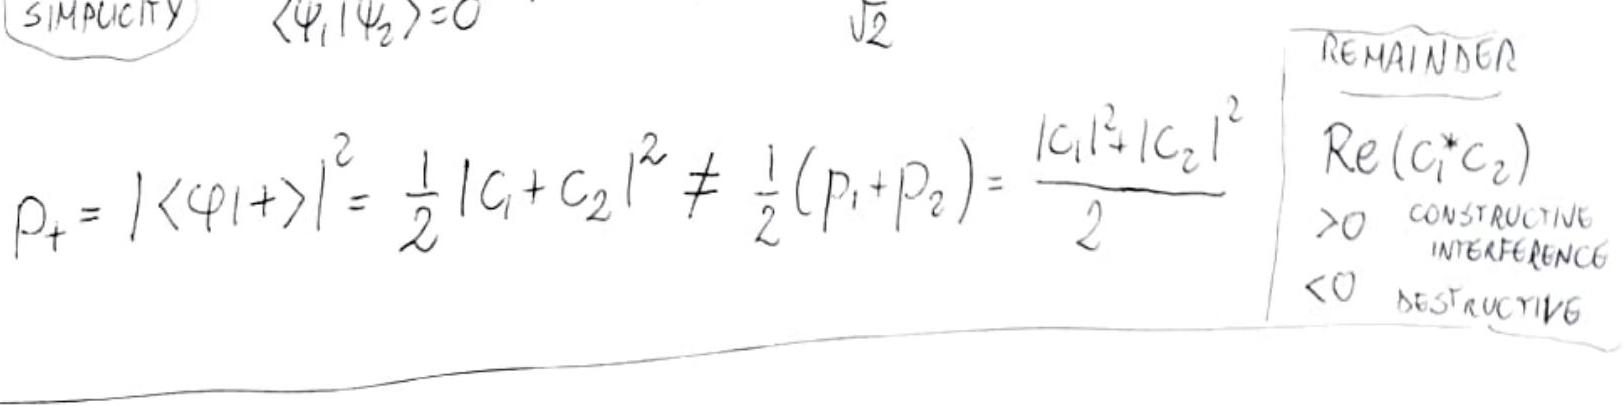
\includegraphics[max width=\textwidth, center]{2025_10_16_f02af6fa434c9f0bcc00g-04}\\
Actually the peobability is

$$
p=\frac{|\langle\psi \mid \varphi\rangle|^{2}}{\langle\psi \mid \psi\rangle\langle\varphi \mid \varphi\rangle} \quad \leqslant \frac{\text { Physical } Q . \Leftrightarrow \begin{array}{l}
\text { INVARIANT UNDER } \\
\text { 'GAUGEE TRALFFORM. }
\end{array}}{\begin{array}{r}
|\psi\rangle \rightarrow \lambda|\psi\rangle \text { WITH } \lambda \in \mathbb{C}(\lambda \neq 0) \\
\text { THUS WE WORK WITH NORMALIZES } \\
\text { GUANTUH STATES }\langle\psi \mid \psi\rangle=\langle\varphi \mid \varphi\rangle=1
\end{array}}
$$

IC Ortmonormal Bases\\
FOR AU PRACTICAL purposes

$$
\operatorname{DIMENSION}(\text { If })=7^{\text {FINITE }}{ }^{\text {COUNTABLE INFINITE }}
$$

Why? Because 10. The lab/sample is finite size\\
(2.) WE WORK AT BOUNSES EWEREY

DEFINE AN ORTHONORMAL BASIS $\left\lvert\, \begin{gathered}\text { n } \\ \uparrow\end{gathered}\right.$ BAND WIOTH

LABEL = ONE OR MORE INTEGERS\\
$\begin{array}{cc}\langle n| n\left\rangle=\delta_{n, n^{\prime}}\right. & \begin{array}{c}\text { KRONECKER } \\ \text { DECTA } \\ \text { NOT SIRAC }\end{array} \\ \text { HIMSENT METRIC } & \end{array} \quad|\psi\rangle=\sum_{\substack{\mid \\ \text { GOES IN HERE }}} C_{n}|n\rangle \quad \begin{gathered}\text { COMPLETE- } \\ \downarrow \\ \text { NESS }\end{gathered}$

\section*{1D OPERATORS}
they are ensomorphisms of ff (linear and H $\rightarrow$ H )\\
NOTATION $\rightarrow \hat{A}|\psi\rangle$\\
WHERE $\langle\varphi \mid \psi\rangle$

$$
\begin{aligned}
& \left\langle\psi_{1}\right| \hat{A}\left|\psi_{2}\right\rangle \stackrel{\text { def }}{=}\left(\left|\psi_{1}\right\rangle, \hat{A}\left|\psi_{2}\right\rangle\right)_{\text {APAIES TO THE RIGHT }} \\
& =\left(\begin{array}{l}
\text { definition of } \\
\text { HERMITIAN } \\
\text { CONGUEATE }
\end{array}\right) \quad\left(\hat{A}^{+}\left|\psi_{1}\right\rangle,\left|\psi_{2}\right\rangle\right)=\left(\begin{array}{c}
\text { HIL BERY } \\
\text { SCALAR } \\
\text { PRODET } \\
\text { PROPERTY }
\end{array}\right) \quad\left(\left|\psi_{2}\right\rangle, \hat{A}^{+}\left|\psi_{1}\right\rangle\right)^{*} \\
& =\left(\left\langle\psi_{2}\right| \hat{A}^{+}\left|\psi_{1}\right\rangle\right)^{*}
\end{aligned}
$$

(2.) Observables \& heasurement\\
an observable is a hecmitian operator $\theta=\theta^{+}$\\
OR MORE PRECISELY $\langle\psi| \theta|\varphi\rangle=(|\psi\rangle, \theta|\varphi\rangle)=(\theta|\psi\rangle,|\varphi\rangle)=\langle\varphi| \theta|\psi\rangle^{*}$

$$
\begin{aligned}
& \theta=\theta^{+} \\
& \text {SPECTRAL } \\
& \text { THEOREM }
\end{aligned}\left\{\begin{array}{ccc}
\theta \text { CAN BE DIAGONALIZED } & \\
& \& & \\
\text { ITS EIGENBASIS IS ORTHOGONAL } & \left(\begin{array}{c}
\text { AT LEAST ONE } \\
\text { H EIGENGASIS } \\
\text { I SORHOGONAL }
\end{array}\right) \\
\text { EIGENVALUES ARE } & \text { REAL } &
\end{array}\right.
$$

$$
G=U D U^{+} \underset{\text { DIAGONAC \& REAL }}{U U^{+}=U^{+} U=\mathbb{1}} \quad U=\sum_{\substack{j \\ \sum_{\text {EIGENVALUES }}}} \eta_{j} \mid J \times\left\langle\varphi_{j}\right| \quad\left(\eta_{1}=\eta_{j}^{*}\right)
$$

$2 A$ The (hard) measurement process\\
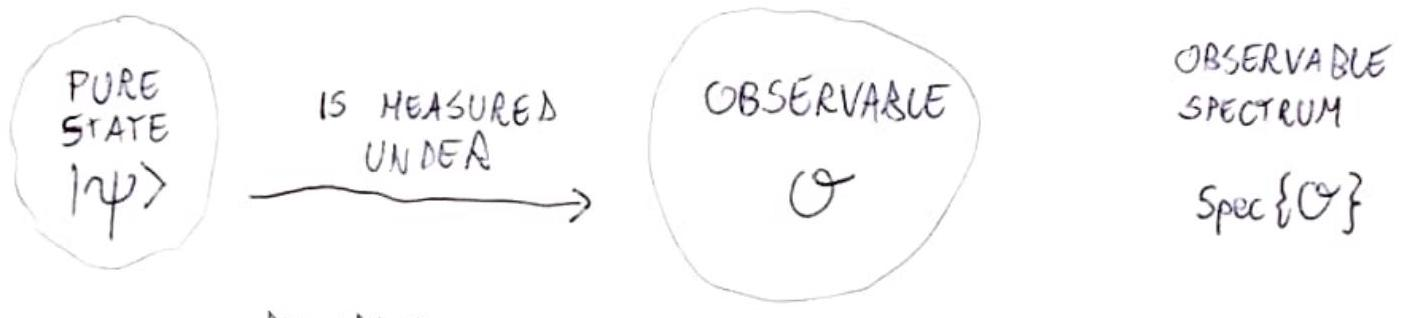
\includegraphics[max width=\textwidth, center]{2025_10_16_f02af6fa434c9f0bcc00g-06}

$$
\begin{gathered}
\text { For EVERY OUTCOME } \\
\lambda \in \operatorname{SPCC}\{\theta\} \\
\Downarrow \\
\Pi_{\lambda} \quad \begin{array}{c}
\text { PROSECTOR OVER } \\
\text { THE EIGENSPACE }
\end{array} \\
\theta \Pi_{\lambda}|\phi\rangle=\Pi_{\lambda}|\phi\rangle \lambda \\
{\left[\Pi_{\lambda}, \theta\right]=0} \\
\Pi_{\lambda}=\Pi_{\lambda}^{2}=\Pi_{\lambda}^{\dagger}
\end{gathered}
$$

$$
\begin{aligned}
& \left.\| \psi_{\lambda}^{\prime}\right\rangle=\frac{\pi_{\lambda}|\psi\rangle}{\sqrt{\langle\psi| \pi_{\lambda}|\psi\rangle}}
\end{aligned}
$$

THIS PROCESS BREAKS TIME REVERSAL (it is FINE BECAUSE it is AN EFFECTIVE PICTURE)

$$
\langle\psi\rangle=\sum_{\lambda}^{1} \lambda p_{\lambda}=\langle\psi|\left(\Sigma \lambda \Pi_{\lambda}\right)|\psi\rangle=\langle\psi| \circlearrowleft|\psi\rangle
$$

$$
\Delta \theta^{2}=\left\langle\theta^{2}\right\rangle-\langle\theta\rangle^{2}
$$

$=\left\langle\left(\theta-\left.\langle\theta\rangle\right|^{2}\right\rangle\right.$

2B operators \& observables so not commute

\section*{$i[A, B]=C$}
$\Delta A \Delta B \geqslant \frac{1}{2}|\langle i[A, B]\rangle| \begin{aligned} & \text { Heisenserg } \\ & \text { uncertanty principle }\end{aligned}$

\section*{in practice}
\begin{center}
\begin{tabular}{|l|l|l|l|l|}
\hline
measure A & A 15 DETERMINES & MEASURE B & B IS DETERMINES & A IS NO HORE DETERMINED \\
\hline
HEISENBERG IS NOT ALWAYS A HARD BOWND & $\Delta p \Delta x \geqslant$ & $\frac{\hbar}{2}$ & HARD BOUND & $\Delta p \rightarrow 0$ MEANS $\Delta x \rightarrow \infty$ \\
\hline
\end{tabular}
\end{center}

\section*{BUT CONSIDER}
$|0\rangle=\binom{1}{0}$

$$
\sigma^{z}=\binom{1}{-1} \quad \sigma^{x}=\left(\begin{array}{ll}
0 & 1 \\
1 & 0
\end{array}\right) \quad \sigma^{y}=\left(\begin{array}{ll}
-i & \\
i &
\end{array}\right)
$$

$|1\rangle=\binom{0}{1}$

$$
\Delta \sigma_{0}^{z} \Delta \sigma_{0}^{x} \geqslant \frac{1}{2}\left|\left\langle\sigma^{y}\right\rangle_{0}\right|
$$

$\Delta \sigma_{0}^{z}=\langle 0|\left(\sigma^{z}-\langle 0| \sigma^{z}|0\rangle\right)^{2}|0\rangle=\langle 0|\left(\sigma^{z}-1\right)^{2}|0\rangle=\sqrt{0}\left(\begin{array}{ll}0 & 0 \\ 0 & 4\end{array}\right)\binom{1}{0}=0$\\
$\Delta \sigma_{0}^{x}=\langle 0|\left(\sigma^{x}-\langle 0| \sigma^{x}|0\rangle\right)^{2}|0\rangle=\langle 0| \sigma^{x^{2}}|0\rangle=\langle 0 \mid 0\rangle=1$\\
$\left\langle\sigma_{0}^{y}\right\rangle_{0}=\frac{10}{10}\binom{-i}{i}\binom{1}{0}=0$\\
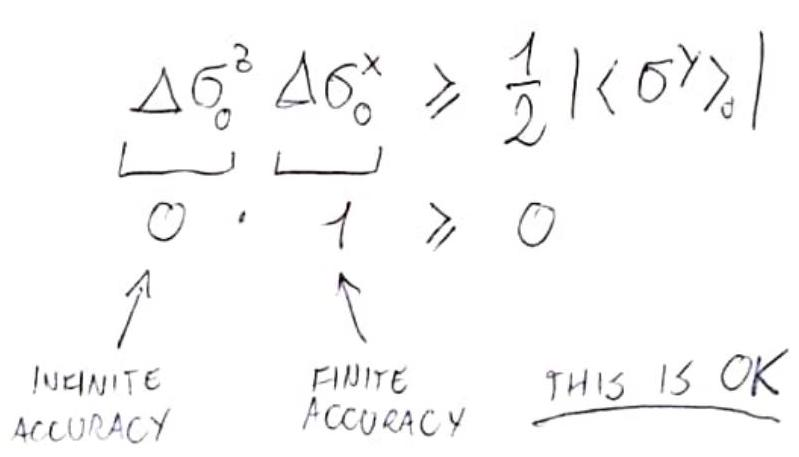
\includegraphics[max width=\textwidth, center]{2025_10_16_f02af6fa434c9f0bcc00g-07}

$$
0 \geqslant 0
$$

WEU, WHATEVER\\
NOT REACY HARD BOUND\\
that's one reason why Q-IN.O MAKES SENSE\\[0pt]
[2C] Physical transformations of a closes quantum system\\
IF A SYSTEM IS CLOSED

$$
\left.\left.|\psi\rangle \rightarrow\left|\psi^{\prime}\right\rangle={ }^{*} I(|\psi\rangle)=|T| \psi\right\rangle\right\rangle
$$

(1) IT STAYS DETERMINISTIC\\
(2) If PRESERVES TOTAL PROBALIKY

$$
\langle T(\psi)| \mathbb{1}|T(\psi)\rangle=\langle\psi| \mathbb{1}|\psi\rangle=1
$$

under physical transformations

$$
(T \psi, T \psi)_{H}=(\psi, \psi)_{H} \quad \forall \psi\left[\begin{array}{c}
\text { THEREE ARE ONCY TWO } \\
\text { POSSIBICITIES }
\end{array}\right.
$$

\section*{T ANTI-UNITARY}
$(T \psi, T \varphi)=(\psi, \varphi)^{*} \quad \forall \psi \varphi$\\
PROBLEM CANNOT CONTINUUJSLY connect with trivital trafo $\mathbb{1}_{.}$ MAOSSIBLE TO ACHIEVE WITH increhental changes

$$
\binom{\text { STIU USEFUL AS A }}{\text { SYMHETRY }}
$$

T UNITARY\\
$(T \psi, T \varphi)=(\psi, \varphi) \quad \forall \psi, \varphi$\\
$1_{\text {THIS IS THE COMMON CASE: }}$ CONTINUOUSLY CONNECTES TO 11 SO TIME EVOLUTION OPERATORS ARE OF THIS CCASS

$$
\left|\psi\left(t^{\prime}>t\right)\right\rangle=U\left(t, t^{\prime}\right)|\psi(t)\rangle
$$

\begin{itemize}
  \item change of reference frame can be both untary and anti-unitary\\
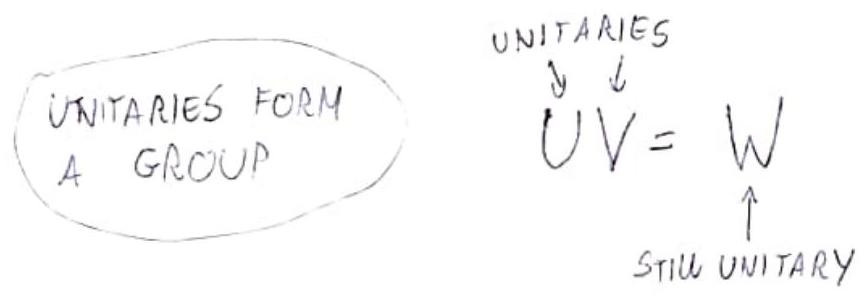
\includegraphics[max width=\textwidth, center]{2025_10_16_f02af6fa434c9f0bcc00g-08(1)}\\
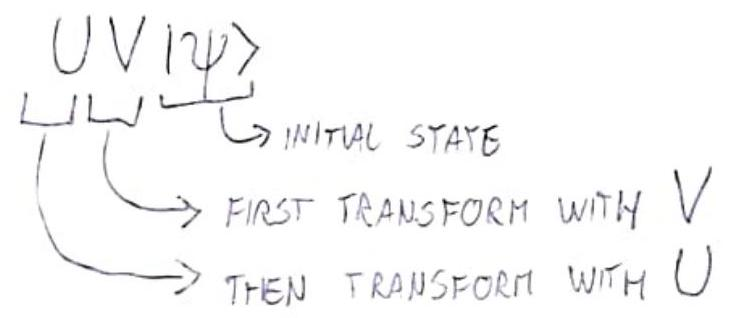
\includegraphics[max width=\textwidth, center]{2025_10_16_f02af6fa434c9f0bcc00g-08(2)}
\end{itemize}

\begin{figure}[h]
\begin{center}
\captionsetup{labelformat=empty}
\caption{hanes sense: stacking hultiple AHYSICA OPS IS STILE A PUYSICAL Op.}
  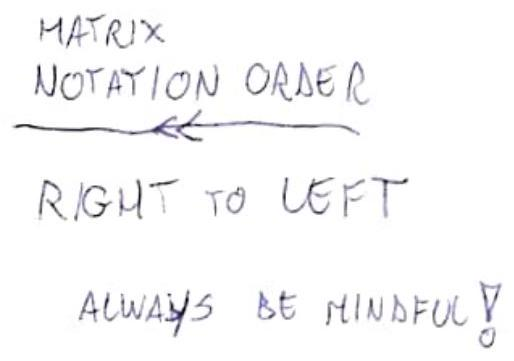
\includegraphics[width=\textwidth]{2025_10_16_f02af6fa434c9f0bcc00g-08}
\end{center}
\end{figure}

(3) Time Evolution

INITIAC CONDITIONS

CLOSES SYSTEM EVO\\
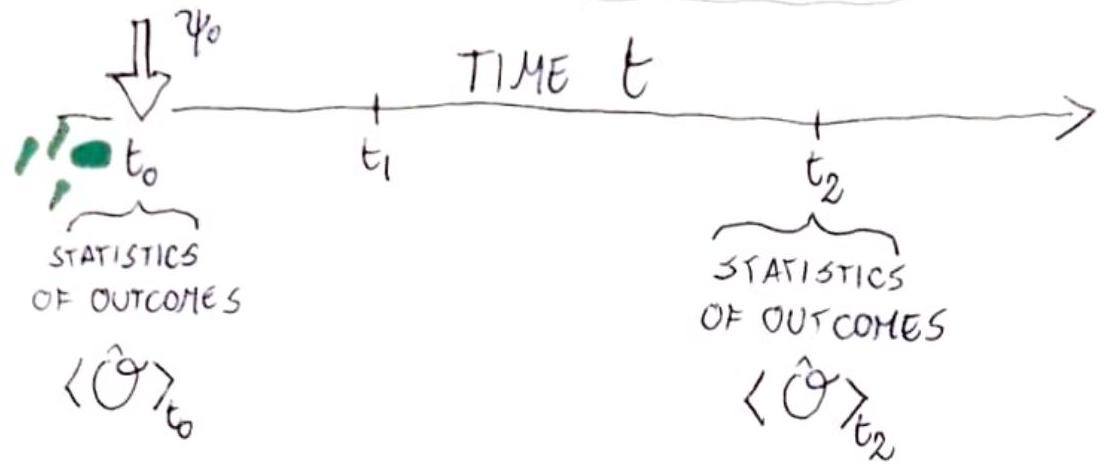
\includegraphics[max width=\textwidth, center]{2025_10_16_f02af6fa434c9f0bcc00g-09}

3A. Schrödinger PICTURE - Evolving Stotes

$$
i \hbar \frac{d}{d t}|\psi\rangle=\hat{H}|\psi\rangle \quad \begin{gathered}
\text { SCHIÖSINGER'S } \\
\text { EQUATION }
\end{gathered} \quad \begin{aligned}
& \text { WHERE } \\
& H=H^{+}
\end{aligned}
$$

holss for EVERY quantum system evo that is\\
(a) PHYSICAL\\
(2) $\operatorname{closes}$\\
(3) FIRST-ORSER SIFFERENTIAL IN TIME\\
(in a way, schrósinger can be relativistic if $H$ is relativistic)

\section*{formal Solutions $H$ is $t$ insepensent}
Ao Diagonalize $H=\sum \varepsilon_{s}\left|\varepsilon_{s} \times \varepsilon_{s}\right| \quad\binom{\text { so THAT }}{H\left|\varepsilon_{s}\right\rangle=\left|\varepsilon_{s}\right\rangle \varepsilon_{s}}$

$$
\left|\varepsilon_{j}\right\rangle \xrightarrow{E V O C U T I O N} e^{-i \varepsilon_{j} t / \hbar}\left|\varepsilon_{j}\right\rangle
$$

B. Expand any intital state $\left|\psi_{0}\right\rangle$ in the eigenbasis

$$
\begin{aligned}
& \left\langle\varepsilon_{j} \mid \psi_{0}\right\rangle=c_{j} \\
& \left|\psi_{0}\right\rangle=\sum_{1} c_{j}\left|\varepsilon_{j}\right\rangle \xrightarrow{\text { EVOLVE }}|\psi(t)\rangle=\sum_{1}^{1}\left|\varepsilon_{j}\right\rangle c_{j} e^{-i \varepsilon_{j} t / \hbar}
\end{aligned}
$$

(BANDWIJTH!),\\
c. formal expression with the matrix exponential

$$
\begin{aligned}
|\psi(t)\rangle & =\underbrace{\left(\sum_{1}\left|\varepsilon_{j}\right\rangle e^{-i \varepsilon_{j} t / \hbar}\left\langle\varepsilon_{j}\right|\right)\left|\psi_{0}\right\rangle}_{\substack{\text { ANS TAS IS INSEES UNTARY } \\
\text { AND ADATIVE } U\left(t_{2}\right) U\left(t_{1}\right)=U\left(t_{1}+t_{2}\right)}} \\
\exp (-i H(t / \hbar) & \left|\psi_{0}\right\rangle
\end{aligned}
$$

DONT FORGET THAT $\exp (A)=1+A+\frac{A^{2}}{2}+\frac{A^{3}}{6}+\ldots=\sum_{j=0}^{\infty} \frac{A^{j}}{j!}$ BUT ALSO $\exp \left(V A V^{+}\right)=V \exp (A) V^{+}$SO ORTENTIMES\\
(e) DIAGONALIEE\\
(2) examentate the eigenvalues

3B. Heisemberg Picture - Evolving OPS

$$
\begin{array}{rlr}
\langle\theta\rangle_{t}=\langle\psi| \theta|\psi\rangle_{t}=\left\langle\psi_{0}\right| \underbrace{+}_{\vec{\theta}(t)}(t) \theta(t)\left|\psi_{0}\right\rangle & \dot{U}(t)=\frac{d}{d t}\left(e^{-i H t / \hbar}\right) \\
\frac{d}{d t} \tilde{\theta}(t)=\dot{U}^{+}(t) \theta U(t)+U^{+}(t) \theta \dot{U}(t) & \left(-\frac{i}{\hbar} H\right) U(t) \\
& =+\frac{i}{\hbar} H U^{+} \theta U-\frac{i}{\hbar} U^{+} \theta U M & {[H, U]=0} \\
\dot{\omega} & =\frac{i}{\hbar}[H, \tilde{\theta}] \quad\left(+U^{+} \dot{\theta} U\right) &
\end{array}
$$

\section*{3C EXAMPLE: DRIVEN 2-LEVEL SYSTEM AND TRANSITIONS}
\begin{center}
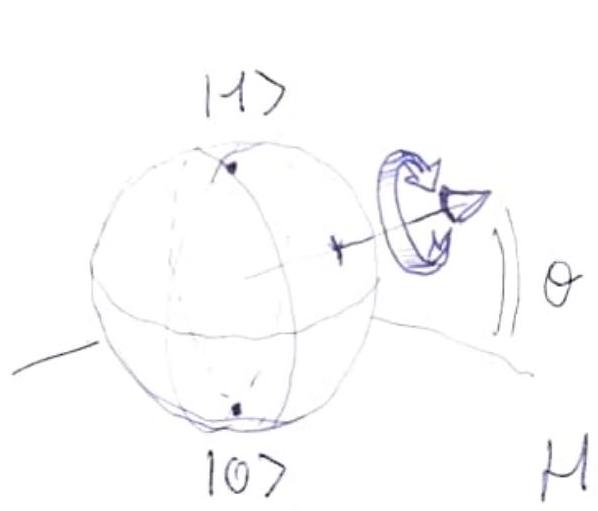
\includegraphics[max width=\textwidth]{2025_10_16_f02af6fa434c9f0bcc00g-11}
\end{center}

$$
\begin{aligned}
& \left|\psi_{0}\right\rangle=0 \\
& \left\lvert\, \begin{array}{l}
\mid=\hbar\left(\Omega \sigma^{x}+\Delta \sigma^{z}\right) \\
\binom{\text { RABI }}{\text { REQ. }} \quad(\text { DETUNING }) \leftarrow \text { WE WIU SEE } \\
\text { WHY THIS } 15 \\
\text { THE CASE }
\end{array}\right.
\end{aligned}
$$

$$
H=\hbar \Omega\left(\begin{array}{ll}
0 & 1 \\
1 & 0
\end{array}\right)+\hbar \Delta\left(\begin{array}{cc}
1 & 0 \\
0 & -1
\end{array}\right)=\hbar\left(\begin{array}{cc}
\Delta & \Omega \\
\Omega & -\Delta
\end{array}\right)
$$

REWRITE $\quad \widetilde{\Omega}=\sqrt{\Omega^{2}+\Delta^{2}} \quad \theta=\arctan \left(\frac{\Delta}{\Omega}\right)$

$$
\begin{aligned}
& \rightarrow \Omega=\Omega \sin \theta \quad \Delta=\tilde{\Omega} \cos \theta \\
& H=\hbar \widetilde{\Omega}(\vec{n} \cdot \overrightarrow{\vec{\sigma}}) \\
& \text { NOTICE THAT }(\vec{n} \cdot \vec{\sigma})^{2}=\mathbb{1}
\end{aligned} \vec{n}=\left(\begin{array}{c}
\cos \theta \\
0 \\
\sin \theta
\end{array}\right) \quad \vec{\sigma}=\left(\begin{array}{c}
\sigma^{x} \\
\sigma^{y} \\
\sigma^{z}
\end{array}\right)
$$

Therefore $\exp \left(-\frac{i \mu t}{\hbar}\right)=\sum_{J} \frac{(-i \tilde{\Omega} t)^{j}}{J!}(\vec{n} \cdot \hat{\vec{\sigma}})^{J}$

$$
\begin{aligned}
= & 1 \sum_{j}^{\text {ever }} \frac{(-i \tilde{\Omega} t)}{j!}+(\vec{n} \cdot \hat{\vec{\sigma}}) \sum_{j}^{\cos } \frac{(-i \Omega t)}{J!} \\
= & \mathbb{1} \cos (\tilde{\Omega} t)+(\vec{n} \cdot \hat{\vec{\sigma}})(-i \sin (\tilde{\Omega} t)) \\
& \cos (\tilde{\Omega} t)\left(\begin{array}{cc}
1 & 0 \\
0 & 1
\end{array}\right)-i \sin (\tilde{\Omega} t)\left(\begin{array}{cc}
\sin \theta & \cos \theta \\
\cos \theta & -\sin \theta
\end{array}\right) \\
\left|\psi_{0}\right\rangle=0= & \binom{1}{0} \\
|\psi(t)\rangle= & \cos (\tilde{\Omega} t)\binom{1}{0}-i \sin (\tilde{\Omega} t)\binom{i \sin \theta}{\cos \theta}
\end{aligned}
$$

probability of measuring (H)

$$
|\langle 1 \mid \psi(t)\rangle|^{2}=\left|\frac{}{01}\binom{\cos \left(\tilde{\Omega}_{t}\right)-i \sin \left(\tilde{\Omega}_{t}\right) \sin \theta}{-i \sin \left(\tilde{\Omega}_{t}\right) \cos \theta}\right|^{2}
$$

$$
=\sin ^{2}(\Omega t) \cos ^{2} \theta
$$

\begin{center}
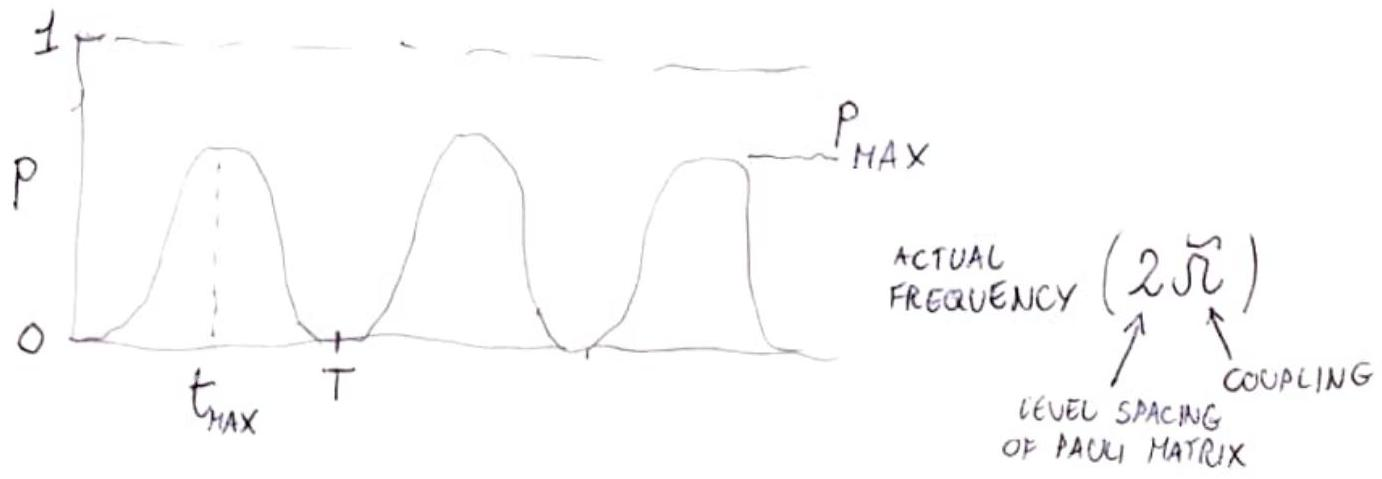
\includegraphics[max width=\textwidth]{2025_10_16_f02af6fa434c9f0bcc00g-12}
\end{center}

$$
t_{\text {MAX }}=(2 J+1) \frac{\pi}{2 \dot{\Omega}}=(2 J+1) \frac{\pi}{2 \sqrt{\Omega^{2}+\Delta^{2}}} \quad T=\frac{\pi}{\Omega}
$$

$\xrightarrow[\substack{\text { TRANSIGION } \\ \text { PROB. }}]{\text { MAX }} P_{\text {MAX }}=\cos ^{2} \theta=\frac{\Omega^{2}}{\Omega^{2}+\Delta^{2}}=\left(1-\frac{\Delta^{2}}{\Omega^{2}+\Delta^{2}}\right)$\\
$\Downarrow$\\
qualitative lesson:\\
To have high transition\\
YOU NEES $\triangle \ll \Omega$\\
(mportant later)


\end{document}